


\subsection{Outline}

The initial solution is to implement a simple MLP neural network which will be trained by raw input data. The intention is to observe the output of the trained network and the network itself and analyse the results to get a sense of direction.\\

\includegraphics[scale=0.55]{initial_approach_outline.png}

\subsubsection{Input Extraction}

The input of the system is pairs of files that compose a DDR game. One of the files is a music file and the other is a steps file. The DDR emulator will parse these 2 files and play the music file in sync with the steps file so the user may play the game.
The music file may come in many different formats such as MP3s, WAVs, AIFFs, and many more. However, all formats are just different representations of raw sound signals and can be readily converted to each other. Some file formats are compressed and will need to be uncompressed. The Wav file format is a standard uncompressed file format. This project converts all input music files to the Wav file format so that only one parser needs to be written. As well, the Wav file format is the easiest to work with because of its very transparent way of data storage.\\

The Wav file format [1] stores a frequency and bitrate followed by a series of sound signals that compose the sounds to be played. The frequency determines the time duration of each sound signal and the bitrate determines how many bits are used to represent each sound signal. The higher these values are, the finer the sound and the more it resembles analog sound. A parser is built to parse a wav file into memory as a list, where each item of the list will represent the amplitude of the sound signal at the time index * (1 / frequency). The wav file may contain more than one channels in which case the resulting list will have one dimension for each channel.
The steps file comes in only one file format (SM file[2]) for the PC emulator. The steps file represent the step data using measures. Each measure will contain data about which arrows will be displayed on the screen at each fraction of the measure (valid fractions are all over powers of 2). The length of each measure is specified in the header of the file, along with other various data that dictate timing factors. A parser is created to parse the steps file into memory as a list, where each item of the list will be a 1 or 0 to represent whether or not a step was present at the exact moment specified by the index. The amount of time each index represents is configurable and will be called with parameters to match that of the sound signal.\\

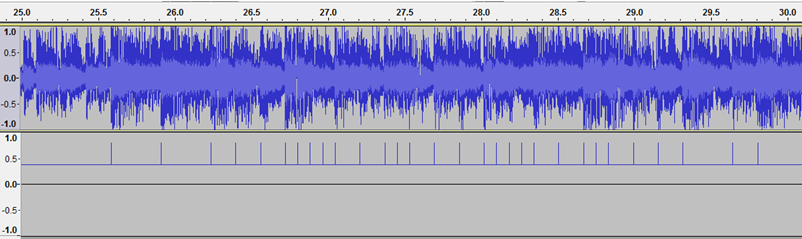
\includegraphics[scale=0.55]{signal_1.png}

Figure x. A visualisation of the sound signal array (top) and the beat signal array (bottom) of a sample input set.


\subsection{Neural Network}

To build a model for predicting beats for specific timeframes, two neural networks were used. The first neural network a custom implemented Multilayer Perceptron network. The second was a feedforward network utilized the third party Keras library wrapping Theano and Tensorflow.

\subsubsection{Custom Implemented Neural Network}
A custom implemented MLP neural network is used to train the data. The configurable parameters are the number of layers, size of each layer, and the input/output size. The neural network is also able to export its current state to file so it can be imported for further training or use.\\

As mentioned previously, the input of the neural network is the raw data of the sound signal and steps signal. A series of sound signals is expected as input and a series of steps signals is expected as output. The entire signal array for both the sound and steps are split up into chunks of 100 signals, and the input/output size of the neural network is configured to 100. For a given song, one epoch consists of running each chunk of 100 signals of the song through the neural network and performing backpropagation.
The algorithm used in the MLP neural network is identical to the backpropagation algorithm discussed in lectures.\\

 At the start of each epoch, each node in the network is initialised with a random weight for each of its parent nodes. When forward propagation of data occurs, the value of the input nodes will be initialised as a chunk of 100 signals of the song. The value of other nodes is then calculated as the summation of the product of each parent node’s value and its respective weight in the current node. The value is then put through a sigmoid activation function before being used by the child nodes. The value of the output nodes is compared to the chunk of 100 signals of the steps. Error is calculated using gradient descent and back propagated. The cumulative error is calculated as the summation of (expected output – actual output) * (1 – output) * (output) across all iterations of the epoch. The weights are updated based on errors and another epoch begins. \\\\
 
\subsection{Keras Library Network Model}

The neural network constructed with Keras was a single layer network with the following configuration:

\begin{itemize}
	\item The input vector was an array of 7 floating point numbers. Each represented a timeframe and the features extracted from it.
	\item One hidden layer with 200 nodes. This layer used a uniform initialization of weights because we had no prior knowledge as to what feature of our input vector was most important
	\item The error function used the stochastic gradient descent algorithm described in class.
	\item The learning rate was 0.01, with a decay of $1e-6$ per epoch.
	\item The output layer was a single node whose value was in $[0,1]$ because the activation function of the one hidden layer was the sigmoid function. This value represented the probability a given timeframe was a beat.
\end{itemize}
 
